\tikzset{every picture/.style={line width=0.75pt}}

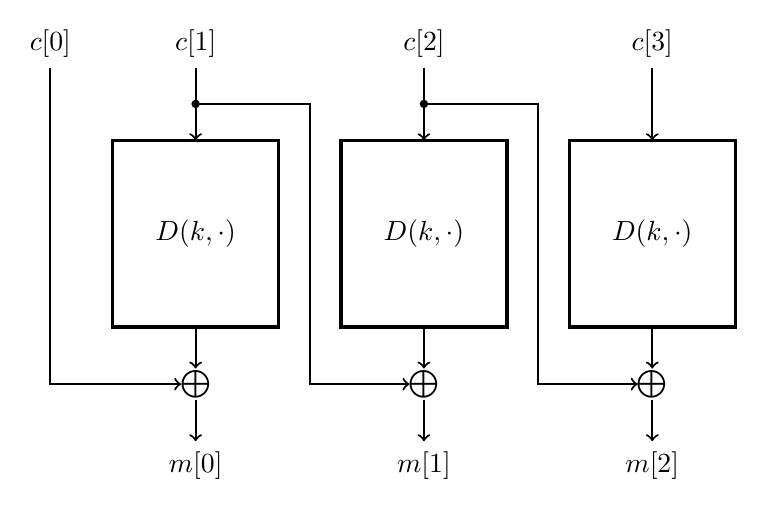
\begin{tikzpicture}[x=0.75pt,y=0.75pt,yscale=-1,xscale=1]

\draw  [line width=1.2]  (90,80) -- (170,80) -- (170,170) -- (90,170) -- cycle ;
\draw  [line width=1.2]  (200,80) -- (280,80) -- (280,170) -- (200,170) -- cycle ;
\draw  [line width=1.2]  (310,80) -- (390,80) -- (390,170) -- (310,170) -- cycle ;

\draw  [->]  (130,45) -- (130,80) ;
\draw  [->]  (130,170) -- (130,190) ;
\draw  [->]  (240,45) -- (240,80) ;
\draw  [->]  (350,45) -- (350,80) ;
\draw  [->]  (130,205) -- (130,225) ;
\draw  [->]  (240,170) -- (240,190) ;
\draw  [->]  (240,205) -- (240,225) ;
\draw  [->]  (350,170) -- (350,190) ;
\draw  [->]  (350,205) -- (350,225) ;
\draw  [->]  (60,45) -- (60,197.5) -- (123,197.5) ;
\draw  [->]  (130,62.5) -- (185,62.5) -- (185,197.5) -- (233,197.5) ;
\draw  [->]  (240,62.5) -- (295,62.5) -- (295,197.5) -- (343,197.5) ;

\draw  [fill={rgb, 255:red, 0; green, 0; blue, 0 }  ,fill opacity=1 ] (128.5,62.5) .. controls (128.5,61.67) and (129.17,61) .. (130,61) .. controls (130.83,61) and (131.5,61.67) .. (131.5,62.5) .. controls (131.5,63.33) and (130.83,64) .. (130,64) .. controls (129.17,64) and (128.5,63.33) .. (128.5,62.5) -- cycle ;
\draw  [fill={rgb, 255:red, 0; green, 0; blue, 0 }  ,fill opacity=1 ] (238.5,62.5) .. controls (238.5,61.67) and (239.17,61) .. (240,61) .. controls (240.83,61) and (241.5,61.67) .. (241.5,62.5) .. controls (241.5,63.33) and (240.83,64) .. (240,64) .. controls (239.17,64) and (238.5,63.33) .. (238.5,62.5) -- cycle ;

\draw (130,125) node    {$D( k,\cdot )$};
\draw (60,41.6) node [anchor=south] [inner sep=0.75pt]    {$c[ 0]$};
\draw (130.03,228.4) node [anchor=north] [inner sep=0.75pt]    {$m[ 0]$};
\draw (240,125) node    {$D( k,\cdot )$};
\draw (130,41.6) node [anchor=south] [inner sep=0.75pt]    {$c[ 1]$};
\draw (240,228.4) node [anchor=north] [inner sep=0.75pt]    {$m[ 1]$};
\draw (350,125) node    {$D( k,\cdot )$};
\draw (240,41.6) node [anchor=south] [inner sep=0.75pt]    {$c[ 2]$};
\draw (350,228.4) node [anchor=north] [inner sep=0.75pt]    {$m[ 2]$};
\draw (130,197.5) node    {$\bigoplus $};
\draw (240,197.5) node    {$\bigoplus $};
\draw (350,197.5) node    {$\bigoplus $};
\draw (350,41.6) node [anchor=south] [inner sep=0.75pt]    {$c[ 3]$};

\end{tikzpicture}